\chapter{Metodologia badań} \label{chap.technology-stack}

\section{Narzędzia, biblioteki, języki programowania}
Do wykonania badań powstała aplikacja internetowa, która udostępnia końcowemu użytkownikowi protokół HTTP. Dzięki temu użytkownik może wykonywać operacje wykorzystujące paradygmat map-reduce bez znajomości platform udostępniających przetwarzanie danych masowych jak również serwisów internetowych. Aplikacja nosi nazwę \textit{big-data-runner}. Aplikacja może być udostępniona na zdalnym serwerze jak również może być uruchomiona lokalnie. Aby uruchomić aplikację jedyne co użytkownik musi posiadać to:
\begin{itemize}
	\item{Wirtualna Maszyna Java w wersji 8\footnote{JVM \url{https://www.java.com/pl/download/}}}
	\item{Scala Build Tool \footnote{SBT \url{http://www.scala-sbt.org/}}}
\end{itemize}
JVM jest odpowiedzialna za środowisko uruchomieniowe aplikacji internetowej. SBT to narzędzie, które umożliwia kompilację całej aplikacji wraz z bibliotekami zewnętrznymi (jeżeli biblioteki nie znajdują się w katalogu lokalnym zostaną pobrane ze zdalnego repozytorium) oraz jej uruchomienie w serwerze aplikacji internetowych \textit{Netty}\footnote{\url{https://netty.io/}}. Z ramę projektową odpowiedzialny jest Play Framework, który umożliwia łatwą i szybką implementację protokołu HTTP dla końcowego użytkownika.
\newpage
Zastosowane języki programowania to:
\begin{itemize}
	\item {Java}
	\item {Scala}
\end{itemize}

Większość kodu aplikacji to Scala - kontrolery, konfiguracja SBT, dostępy do serwisów zewnętrznych, wywoływanie interfejsu programistycznego Spark. Java została wykorzystana podczas obsługi API\footnote{Application Programmer Interface} platformy Hadoop tworząc w ten sposób własne API, które mogło być wykorzystane w kontrolerach napisanych w Scali.

\section{Architektura aplikacji}
Architektura aplikacji big-data-runner jest przedstawiona na rysunku \ref{fig:@=big-data-runner_arch}. 
\begin{figure}[!htb]
	\centering
	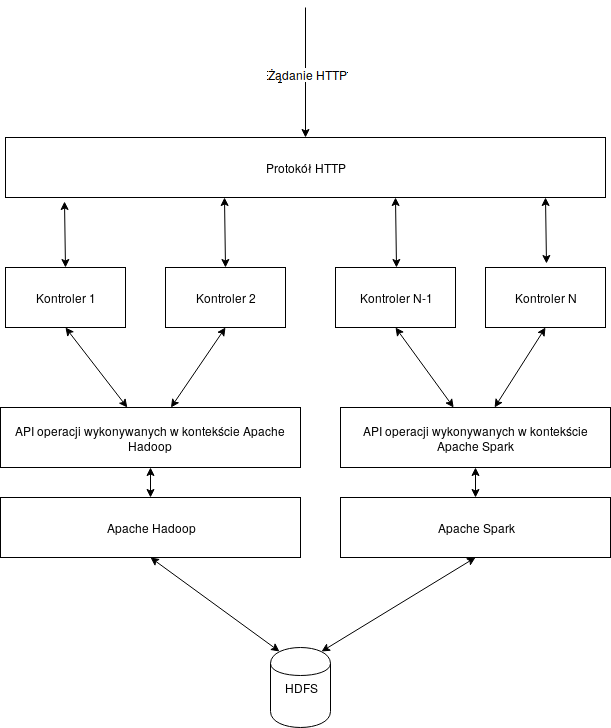
\includegraphics[scale=0.4]{big-data-runner-architecture.png}
	\caption{Architektura big-data-runner}
	\label{fig:@=big-data-runner_arch}
\end{figure}
\newline Podczas użytkowania użytkownik wysyła żądanie HTTP do aplikacji. Cały mechanizm obsługi żądania oraz odpowiedzi jest zaimplementowany w ramie projektowej Play! Za żądania odpowiedzialne są kontrolery, które wykonują logikę biznesową aplikacji. W zależności od adresu żądania wywołanego przez użytkownika uruchamiany jest odpowiedni kontroler, który wywołuje daną operację na platformie obliczeniowej. W zależności od tego czy operacje są wywoływane w kontekście platformy Hadoop czy Spark, używane są odpowiednio języki programowania: Java, Scala. Z racji iż aplikacja integruje dwie platformy obok siebie możemy uznać, że kontrolery są częścią aplikacji, które wysyłają \textit{driver program}\footnote{Program sterujący - \url{http://spark.apache.org/docs/latest/cluster-overview.html}} do platformy Hadoop lub Spark. W dokumentacji Apache Hadoop możemy spotkać się z określeniem \textit{Job Configuration}\footnote{Konfiguracja pracy - \url{https://hadoop.apache.org/docs/r2.7.3/api/org/apache/hadoop/mapreduce/Job.html}}. Po wysłaniu odpowiednich instrukcji następuje wykonywanie obliczeń przez daną platformę. Same platformy są dołączone do aplikacji jako biblioteki zewnętrzne. Są integrowane przez narzędzie budujące aplikację SBT. Jednym elementem systemu przetwarzania danych masowych, który nie jest zintegrowany z aplikacją jest HDFS - warstwa odpowiedzialna za przechowywanie danych. HDFS może być umiejscowiony na zdalnym serwerze bądź obok samej aplikacji. Może być pobrany pod adresem: \url{http://hadoop.apache.org/releases.html}. W przeprowadzonych badaniach została użyta wersja 2.8.0. Adres HDFS jest zdefiniowany we właściwościach aplikacji, które znajdują się w pliku \path{<application-root>/conf/application.conf}. Dzięki temu w łatwy sposób administrator aplikacji może zmieniać adres źródła danych.
\section{Interfejs końcowy użytkownika}\label{sec:user_interfaces}
Żądania HTTP obsługują trzy rodzaje operacji, które można wykonać na platformach równoległych:
\begin{itemize}
	\item {Zliczanie ilości wystąpień poszczególnych fraz tekstowych (oddzielonych spacją) znalezionych w źródle danych oraz zapisu wyniku do pliku}\footnote{\textit{Word Count}}
	\item {Zliczanie ilości linii zawierających frazę tekstową zdefiniowaną przez użytkownika}\footnote{\textit{Filter}}
	\item {Odrzucenie linii zawierających frazę tekstową zdefiniowaną przez użytkownika oraz zapisanie wyniku do pliku}\footnote{\textit{Reject}}
\end{itemize}
Użytkownik może wybrać następujące punkty obsługi żądania:
\begin{enumerate}
	\item{\url{<hostname>/api/spark/wordcount}}
	\item{\url{<hostname>/api/spark/wordOccurrence/<string> }}
	\item{\url{<hostname>/api/spark/wordReject/<string> }}
	\item{\url{<hostname>/api/hadoop/wordcount}}
	\item{\url{<hostname>/api/hadoop/wordOccurrence/<string>}}
	\item{\url{<hostname>/api/hadoop/wordReject/<string> }}
\end{enumerate}
Punkty od 1 do 3 obsługują platformę Spark. Punkt 1 jest odpowiedzialny za zliczanie wystąpień poszczególnych fraz, punkt 2 za zliczanie wystąpień danej frazy w linii. Punkt 3 odrzuca te linie, które zawierały frazę zdefiniowaną przez użytkownika. Odpowiednio punkty 4, 5, 6 są odpowiedzialne za te same operacje z tą różnicą, że są uruchamiane na platformie Hadoop.  

\section{Dostęp do serwisów zewnętrznych}\label{sec:twitter-api}
Aplikacja posiada również dostęp do jednego serwisu zewnętrznego jakim jest \textit{Twitter Developer API}\footnote{\url{https://dev.twitter.com/}}. Funkcjonalność ta została zaimplementowana, gdyż Twitter jest doskonałym źródłem danych masowych. Na podstawie danych zebranych poprzez Twitter Developer API zostały wykonane badania dotyczące szybkości obu platform. Sam proces zbierania danych jest zaimplementowany poprzez wykorzystanie \textit{Spark Streaming}\footnote{\url{http://spark.apache.org/streaming/}}. Dzięki temu użytkownik jest w stanie zbierać dane "na żywo". Oznacza to, że otwierany jest potok z danymi, które są zapisywane cyklicznie do HDFS. Cykl zapisu to okres czasu co jaki ma wystąpić zapis. W przypadku aplikacji big-data-runner jest to \textbf{360 sekund}. Dzięki takiemu podejściu możliwe jest zbieranie wielkich ilości danych bez ryzyka, iż niestabilne połączenie internetowe uszkodzi dane, bądź całkowicie uniemożliwi zapis. Aby móc skorzystać z Twitter Developer API wymagane są odpowiednie uprawnienia. Uprawnienia są przyznawane dla pary: użytkownik - aplikacja. Dane uprawnień znajdują się w pliku \path{<application-root>/conf/twitter.conf}. Konfiguracja uprawnień jest zapewniona przez bibliotekę \textit{Twitter4J}.\footnote{\url{http://twitter4j.org}}
\newline Dane mogą być zbierane poprzez dwa punkty obsługi żądania aplikacji:
\begin{enumerate}
	\item{\url{<hostname>/api/spark/live/list/start}}
	\item{\url{<hostname>/api/spark/live/list/stop}}
\end{enumerate}
Punkt nr 1 odpowiada za wystartowanie strumieniowania danych do HDFS skonfigurowanego z aplikacją. Punkt nr 2 kończy operację strumieniowania. Zakończenie strumieniowania nie jest natychmiastowe, aplikacja czeka aż cykl zapisu zostanie ukończony. Zasada działania jest taka sama jak w przypadku punktów obsługi wymienionych w sekcji \ref{sec:user_interfaces} z jednym wyjątkiem - przed zatwierdzeniem operacji na platformie Spark, wykonywana jest konfiguracja dostępu do Twitter Developer API. Następnie rozpoczyna się strumieniowanie danych.
